\documentclass[11pt]{article}
\usepackage{graphicx}
\usepackage{float}

\begin{document}
\title{Partial Differential Equations}
\author{Colt Bradley}
\date{}
\maketitle

\section{Part 1}

We are aiming to develop a method to solve partial differential equations, namely the wave equation throughout this lesson. First, we apply a finite difference scheme, which involved dividing both time and space into $N$ segments, giving us $N+1$ nodes. Combining these nodes and with certain boundary conditions, we can numerically solve the PDE. 

For the solution depicted in the graph, we have used a Gaussian as the initial position. To verify that the wave speed $c = 50.0m/s$, we can visually see that after 5 iterations the central peak reaches the bottom. At this point, the peak is at $\pm 2.5 m$. By timesteps, 5 iterations is $.01 s$, and $2.5/.01 = 50.0$

\begin{figure}[H]
\centering
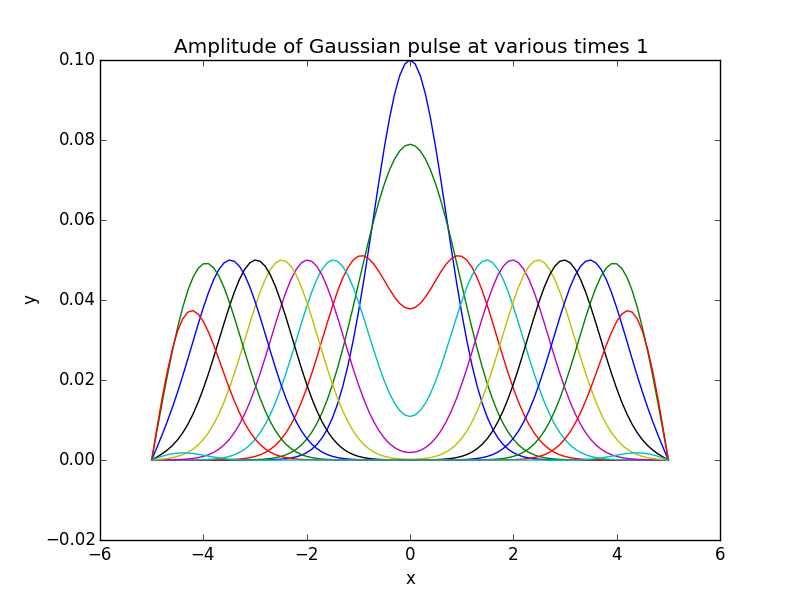
\includegraphics[scale=.5]{part1.png}
\end{figure}


\section{Part 2}

Now, we solve the system a different way. This method is very similar to the second-order Runge-Kutta, and as expected it yield the same results with the same initial conditions as the first. 

To find the Courant condition, we adjust $\eta$ in front of $\eta \Delta x/\Delta c$. Breakdown begins when $\eta = .54$.

\begin{figure}[H]
\centering
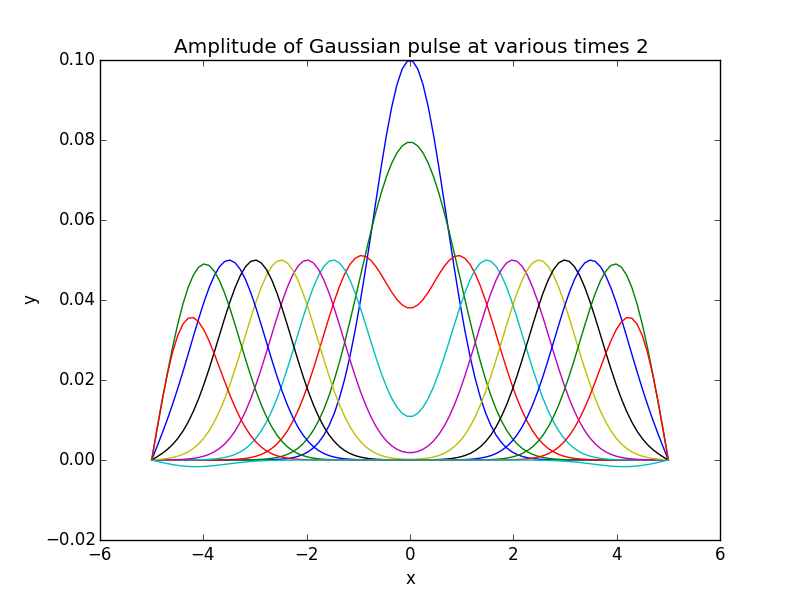
\includegraphics[scale=.5]{part2.png}
\end{figure}

\section{Part 3}

For the last part, we change the initial conditions to add an initial velocity to the wave. The wave propagates to the right, hits the wall, then switches to a negative amplitude and begins moving the opposite direction. We could expect this, as this is how a wave moving down a string physically behaves. 

\begin{figure}[H]
\centering
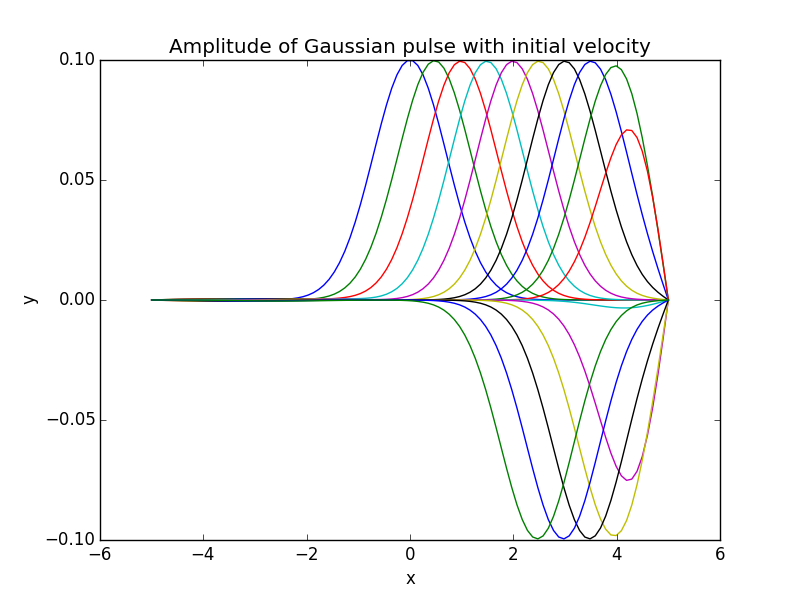
\includegraphics[scale=.5]{part3.png}
\end{figure}

\section{Code}
\subsection{Part 1 Code}
\begin{verbatim}
# Solve the PDE for waves on a string
import pylab as pl
import numpy as np

# Parameters
c = 50.0
xa = -5.0
xb = 5.0
A = 0.1
sigma = 1.0

# Set up grid
N = 100  # number of space intervals
nts = 200  # number of timesteps
plt = 20 # number of timesteps between plots
dx = (xb - xa)/N
dt = 0.25*dx/c
cdtoverdxsqr = (c*dt/dx)**2
x = np.linspace(xa,xb,N+1)

# arrays
y = np.zeros(N+1)
ym = np.zeros(N+1) # "y_minus" = y at previous timestep
yp = np.zeros(N+1) # "y_plus"  = y at next timestep

# initial data
for i in range(0,N+1,1):
    ym[i] = A*np.exp(-(x[i]/sigma)**2)
pl.close()
pl.plot(x,ym)

# take the first timestep
y = np.copy(ym)
n = 1
time = dt

# Evolve
while n < nts:
    for i in range(1,N,1):
        yp[i] = 2.0*y[i] - ym[i] + cdtoverdxsqr*(y[i+1] - 2.0*y[i] + y[i-1])
    ym = np.copy(y)
    y = np.copy(yp)
    n = n + 1
    time = time + dt
    if (plt*(n/plt) == n): #plot every plt timesteps
        pl.plot(x,y)
        print n, time

pl.title("Amplitude of Gaussian pulse at various times 1")
pl.xlabel('x')
pl.ylabel('y')
pl.savefig("part1.png")
pl.show()

\end{verbatim}
\subsection{Part 2 Code}
\begin{verbatim}
# Solve the PDE for waves on a string
import pylab as pl
import numpy as np

# Parameters
c = 50.0
xa = -5.0
xb = 5.0
A = .1
sigma = 1.

# Set up grid
N = 100  # number of space intervals
nts = 200  # number of timesteps
plt = 20 # number of timesteps between plots
dx = (xb - xa)/N
dt = 0.25*dx/c
x = np.linspace(xa,xb,N)

# arrays
y = np.zeros(N)
ym = np.zeros(N) # "y_minus" = y at previous timestep
yp = np.zeros(N) # "y_plus"  = y at next timestep
v = np.zeros(N)
vm = np.zeros(N) # "v_minus" = v at previous timestep
vp = np.zeros(N) # "v_plus"  = v at next timestep

# initial data
for i in range(0,N,1):
    y[i] = A*np.exp(-(x[i]/sigma)**2)
pl.close()
pl.plot(x,y)

# take the first timestep
ym = np.copy(y)
n = 1
time = 0

#populate initial arrays

# Evolve
while n < nts:
    #first step
    ym[:] = y[:] +(dt/2.)*v[:]
    vm[1:-1] = v[1:-1] +(dt/2.)*(c**2.)*((y[2:]-2.*y[1:-1]+y[:-2])/dx**2.)
    #second step
    yp[:] = y[:]+dt*vm[:]
    vp[1:-1] = v[1:-1] +(dt)*(c**2.)*((ym[2:]-2.*ym[1:-1]+ym[:-2])/dx**2.)
    
    v = np.copy(vp)
    y = np.copy(yp)
    n = n + 1
    time = time + dt
    if (plt*(n/plt) == n): #plot every plt timesteps
        pl.plot(x,yp)
        print n, time
       
pl.title("Amplitude of Gaussian pulse at various times 2")
pl.xlabel('x')
pl.ylabel('y')
pl.savefig("part2.png")
pl.show()

\end{verbatim}
\subsection{Part 3 Code}
\begin{verbatim}
# Solve the PDE for waves on a string
import pylab as pl
import numpy as np

# Parameters
c = 50.0
xa = -5.0
xb = 5.0
A = .1
sigma = 1.

# Set up grid
N = 100  # number of space intervals
nts = 300  # number of timesteps
plt = 20 # number of timesteps between plots
dx = (xb - xa)/N
dt = 0.25*dx/c
x = np.linspace(xa,xb,N)

# arrays
y = np.zeros(N)
ym = np.zeros(N) # "y_minus" = y at previous timestep
yp = np.zeros(N) # "y_plus"  = y at next timestep
v = np.zeros(N)
vm = np.zeros(N) # "v_minus" = v at previous timestep
vp = np.zeros(N) # "v_plus"  = v at next timestep

# initial data
for i in range(0,N,1):
    y[i] = A*np.exp(-(x[i]/sigma)**2)
for i in range(0,N,1):
    v[i] = (2*A*c*x[i]/sigma**2)*np.exp(-(x[i]/sigma)**2)
pl.close()
pl.plot(x,y)

# take the first timestep
ym = np.copy(y)
vm = np.copy(v)
n = 1
time = 0

#populate initial arrays

# Evolve
while n < nts:
    #first step
    ym[:] = y[:] +(dt/2.)*v[:]
    vm[1:-1] = v[1:-1] +(dt/2.)*(c**2.)*((y[2:]-2.*y[1:-1]+y[:-2])/dx**2.)
    #second step
    yp[:] = y[:]+dt*vm[:]
    vp[1:-1] = v[1:-1] +(dt)*(c**2.)*((ym[2:]-2.*ym[1:-1]+ym[:-2])/dx**2.)
    
    v = np.copy(vp)
    y = np.copy(yp)
    n = n + 1
    time = time + dt
    if (plt*(n/plt) == n): #plot every plt timesteps
        pl.plot(x,yp)
        print n, time
       
pl.title("Amplitude of Gaussian pulse with initial velocity")
pl.xlabel('x')
pl.ylabel('y')
pl.savefig("part3.png")
pl.show()

\end{verbatim}


\end{document}